% !TEX root =  ../master.tex
\chapter{Nutzerhandbuch} %TODO: Das hier eventuell nochmal überarbeiten und kürzen?
Bei der Endwicklung der Anwendung haben wir großen Wert auf eine intuitive Gestaltung der \ac{GUI} und der \ac{UX} gelegt.
% TODO: ist das eine nicht-funktionale Anforderung?
Ziel war es, eine Anwendung zu gestalten, deren Nutzer die Anwendung ohne Erklärung verstehen.
Dennoch möchten wir in diesem Kapitel ein Referenzhandbuch erstellen.
In diesem Kapitel wird beschrieben, wie Nutzer die Anwendung verwenden können.

% TODO: Bilder müssen überall rein
\section{Öffnen der Anwendung}
Die Anwendung kann jederzeit \href{https://dhbwlearning.web.app}{\enquote{dhbwlearning.web.app}} geöffnet werden.
Wie jede andere Webapplikation kann dies über jedes Gerät, welches über eine Internetverbindung verfügt durch einen Webbrowser geöffnet werden.
Das heißt, die Anwendung steht den 24\,h pro Tag bereit und kann von allen Studenten und Dozenten verwendet werden.

\section{Login}
Nach dem Öffnen der Anwendung wird der Nutzer in der Regel aufgefordert sich einzuloggen.
In \autoref{fig:login} ist die Anmeldeseite dargestellt.

\begin{figure}[h]
    \centering
    \includegraphics[width=.7\textwidth]{img/Login}
    \caption{Login-Maske}
    \label{fig:login}
\end{figure}

Für die Anmeldung muss der Nutzer die Email-Adresse zu seinem Account, sowie das entsprechende Passwort angeben.
Setzt der Nutzer einen Hacken bei \enquote{Remember me}, so wird der Nutzer beim nächsten starten der Anwendung nicht um ein Password gebeten und wird automatisch in seinen Account eingeloggt.

Sollte der Nutzer noch keinen Account haben kann er auf \enquote{Register} klick, um sich selbst für die Nutzung der Anwendung zu registrieren.
Genaueres zur Registrierung sind in \autoref{sec:registrierung} beschrieben.

Sollte der Nutzer bereits einen Account haben und nur das Password zu diesem vergessen haben gibt es neben dem Password-Feld einen \enquote{Forgot Password?}-Button.
Dieser leitet den Nutzer zu einem Password-Vergessen-Formular weiter, welches in \autoref{sec:passwordVergessen} beschrieben ist.

Hat der Nutzer eine korrekte Email- und Passwordkombination eingetragen und auf \enquote{Login} geklickt, wird der Nutzer auf das Dashboard (vgl. \autoref{sec:dashboard}) weitergeleitet.
Andernfalls wird der Nutzer freundlich darauf hingewiesen, dass das Password nicht korrekt ist.



\section{Registrierung}\label{sec:registrierung}
Die Registrierungs-Maske dient dazu, einen neuen Nutzer in der Anwendung anzulegen.
Damit sich Nutzer registrieren können müssen sie eine Email-Adresse sowie ein Password wählen.
Der Nutzer kann hierbei eine beliebige, sogar eine Wegwerf-Email verwenden.
Die Email wird intern lediglich für Authentifizierungszwecke benötigt.
Das heißt die Email wird nur für das Login und für den Fall, dass ein Nutzer sein Passwort vergessen hat benötigt (vgl \autoref{sec:passwordVergessen}).
Verwendet der Nutzer eine Wegwerf-Email kann der die Anwendung wie gewohnt nutzen, verliert aber die Möglichkeit sein Passwort zurückzusetzen.

Das Password kann frei gewählt werden, solange es mindestens 6 und maximal 50 Zeichen hat.
Es gibt keine weiteren Einschränkungen, da wir der Meinung sind, dass aufwändige Passwortvorgaben eine schlechte \ac{UX} ergibt.
Dennoch sollten Nutzer Passwörter verwenden, die allgemein als sicher gelten.
% TODO: Vielleicht nochmal sagen, das wir sicher sind, weil firebase google auth?
Um zu verhindern, dass sich der Nutzer bei seinem Passwort vertippt hat, muss das Passwort ein zweites Mal bestätigt werden.

Schließlich muss der User den Nutzungsbedingungen zustimmen.
% TODO:

Sollte der Nutzer bereits einen Useraccount besitzen kann er jederzeit durch einen klick auf \enquote{Log in} zur Login-Maske zurückkehren.

Ist alles korrekt ausgefüllt kann der Nutzer durch klick auf \enquote{Registrieren} die Anmeldung abschließen und wird automatisch eingeloggt.

\begin{figure}[h]
    \centering
    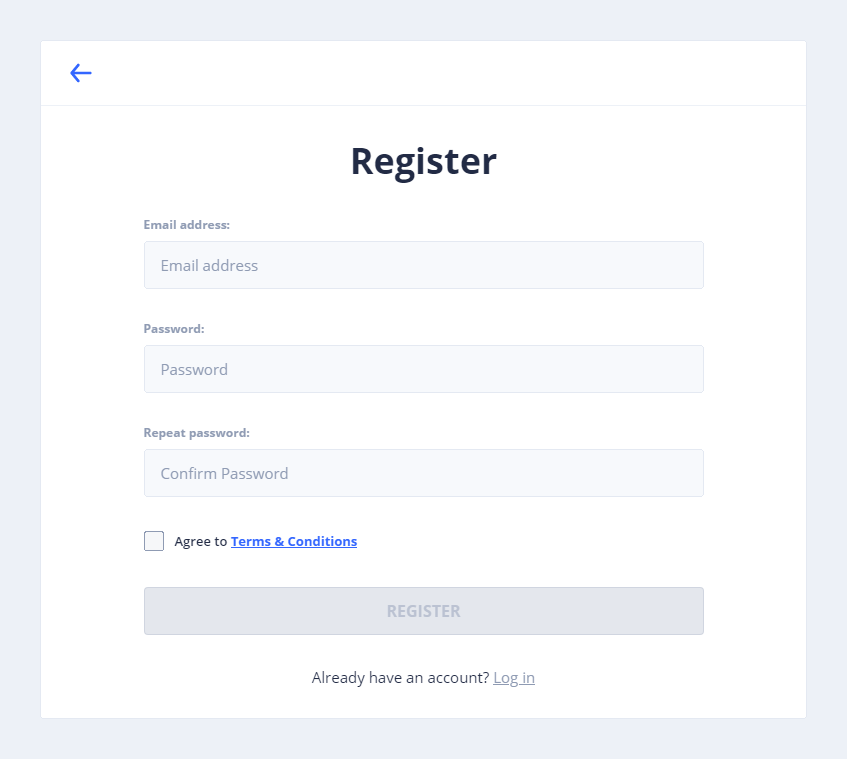
\includegraphics[width=.7\textwidth]{img/register.png}
    \caption{Registrierungs-Maske}
    \label{fig:registrierung}
\end{figure}


\section{Password-Vergessen}\label{sec:passwordVergessen}
Die Password-Vergessen-Funktion dient zum Zurücksetzen des Passwortes.
Möchte der Nutzer sein Password zurücksetzen und erneut Zugang zu seinem Account bekommen kann der Nutzer jederzeit seine Email in das Password-Vergessen-Feld eingeben.

\begin{figure}[h]
    \centering
    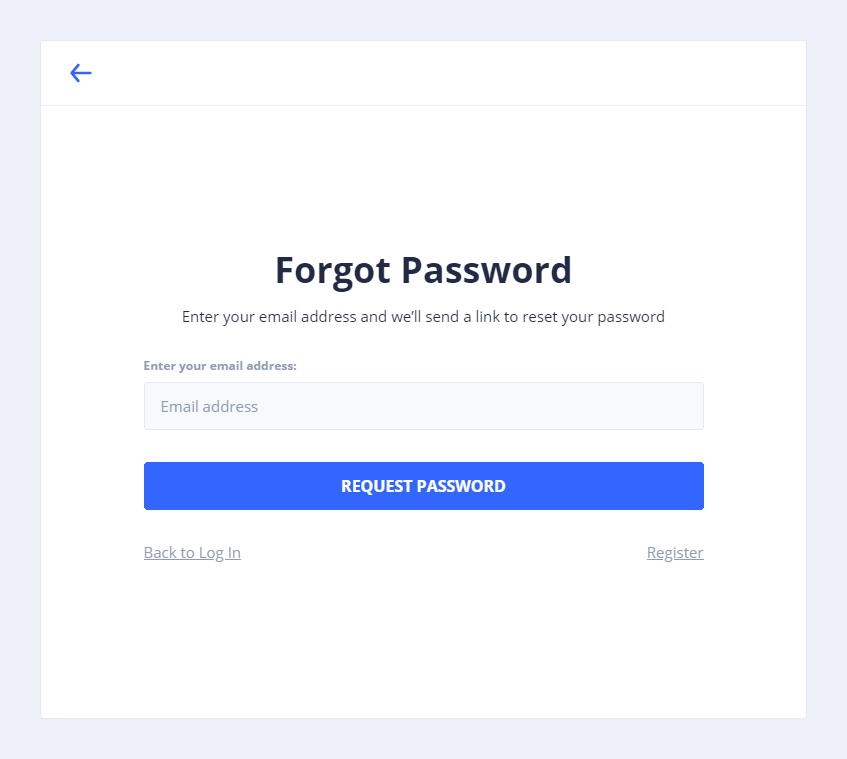
\includegraphics[width=.7\textwidth]{img/passwordReset.png}
    \caption{Password-Vergessen-Maske}
    \label{fig:passwordVergessen}
\end{figure}

Nachdem der Nutzer auf \enquote{Request Password} geklickt hat wird automatisch eine Email an die angegebene Email-Adresse gesendet.
Die Email enthält einen Link, mithilfe dem der Nutzer sein Passwort ändern kann.
Der Link leitet den Nutzer auf die in \autoref{fig:passwordVergessen} dargestellte Maske in der der Nutzer sein Passwort ändern kann.
Hat der Nutzer sein Passwort geändert wird der zu einem erneuten Login auf die Login-Maske geleitet.

Anzumerken ist, dass der Link zum Passwort ändern nur einmal gültig ist.
Sollte das Passwort bereits geändert worden sein, muss eine neue Email angefordert werden.
Dies verhindert, dass unberechtigte Personen die Email mitlesen können und das Passwort erneut ändern könn

% TODO: Muss man hier jede kleinigkeit schreiben? also das email auch wirklich eine email sein muss?


\begin{figure}[h]
    \centering
    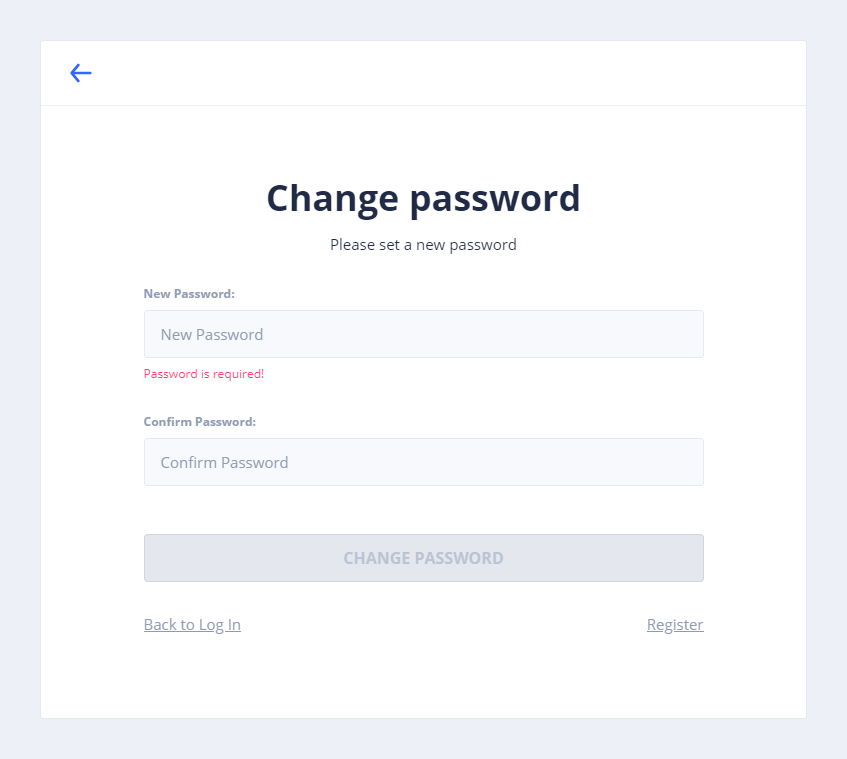
\includegraphics[width=.7\textwidth]{img/passwordReset2.png}
    \caption{Password-Aktualisieren-Maske}
    \label{fig:passwordVergessen2}
\end{figure}

% ..


\section{Dashboard}\label{sec:dashboard}
... siehe User Journey


\section{Karteikarten}\label{sec:Karteikarten} % TODO: Bilder
Index-Cards stellen eine Karteikarten-Funktion dar.
Im Nutzer-Interface werden Karten ähnlich zu einem realen Karteikasten hintereinander dargestellt.
Jede Karte zeigt zunächst die Frage an.
Solle man die Antwort zu der Frage nicht wissen oder sich kontrollieren wollen, kann man mithilfe des Pfeils im Eck einer jeden Karte die Antwort einblenden.
Anschließend können die Karten mit den Buttons am unteren Bildschirmrand als gewusst und nicht gewusst markiert werden.
Durch die Zahlen an diesen Buttons kann der Nutzer leicht ablesen, wie viele Karten der Nutzer bereits wusste.
Karten können aber auch durch einfaches ziehen der Karten zu gewusst oder nicht gewusst verschoben werden.
Dies erleichtert die Handhabung.

Wurden alle Karteikarten beantwortet bekommt der Student direkt Feedback, wieviel Prozent aller Fragen er richtig beantworten konnte.
% TODO: Zusätzlich bekommt er angezeigt, welche Karten er nocheinmal auffrischen sollte
% TODO: Erstellung


\section{TODOs}\label{sec:TODOs} % TODO:
TODOs stellen einen elementaren Bestandteil einer Ausbildung dar.
Schon in der Schule mussten Schüler eine Hausaufgabenheft oder Ähnliches führen um einen Überblick über ihre TODOs zu haben.
Auch im Studium gibt es Unzähliche TODOs, ...

TODOs können mithilfe des \enquote{Floating Action Button (FAB)} im rechten unterem Eck erstellt werden. % https://material.io/components/buttons-floating-action-button#usage
Fabs stellen die primäre Action einer Ansicht, die konstruktiv ist und zu dem Inhalt der Ansicht passt.
Inner


% TODO: Die Material Principien besser herausarbeiten  https://material.io/components/dialogs#usage
Nach dem Klick öffnet sich ein Modal, in dem alle relevanten Todos eingetragen werden können.
Todos zeichnen sich durch einen Titel und eine optionale Beschreibung, sowie eine optionale Deadline aus.
Sofern eine Deadline angegeben ist, wird dieses Todo in den Kalender über der Todo Übersicht dargestellt.
Je roter ein Tag ist, desto mehr Todos müssen an diesem Tag erledigt sein.
Der Kalender zeigt stets den Zeitraum zwischen Anfang des letzten Monates und Ende der nächsten zwei Monate  an.
% TODO: ?
Todos können schnell und einfach durch klicken auf die Checkbox vor einem Todo abgehackt werden.





% TODO: Das hier schreiben, wenn da tatsächlich was implementiert ist

% TODO: Kurs einschreibung, ...



\section{Files}
Die \enquote{Files}-Maske dient zur Verwaltung von Dokumenten.
% TODO: Das in Konzeption verschieben?
Momentan müssen Dokumente umständich an Studenten weitergegeben werden.
In der Regel werden Dokumente an die Studiengangsleiter geschickt, welche die Dokumente anschließend weiterverteilen.
Das Problem ist, dass zuerst die Email-Adressen dieser ausgetauscht werden müssen und diese einen zusätzlichen Aufwand haben.
So sind neue oder korrigierte Dokumente nur schwer auszutauschen.
Auch Dokumente, die während einer Vorlesung verteilt werden müssen, erzeugen eine Zeitdifferenz.
Dazu kommt, das dieser Workflow nicht immer gleich ist.
Oft bekommen verschiedene Schülter unterschiedliche Informationen.
In einigen Fällen wird auch Moodle für die Dateiablage verwendet.

Aus diesem Grund wird ein einheitliches System benötigt, in dem Dateien abgelegt werden können.

\begin{figure}[h] 
    \centering
    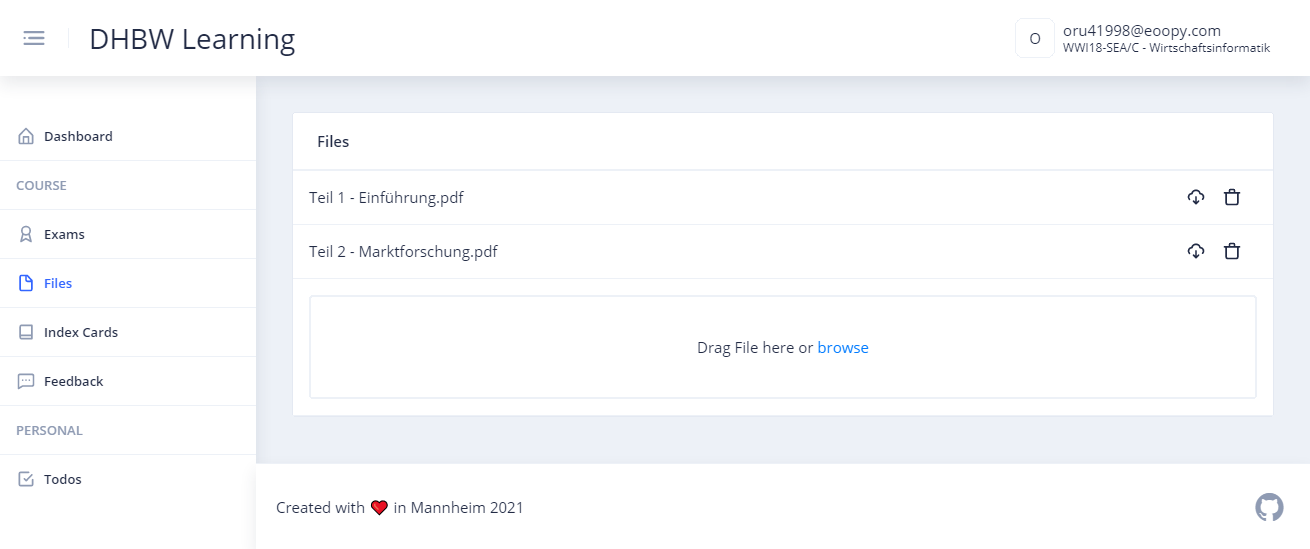
\includegraphics[width=\textwidth]{img/Files.png}
    \caption{Files-Maske}
    \label{fig:files}
\end{figure}

Das in \autoref{fig:files} dargestellte Datenmanagementsystem erleichtert dies, da Dokumente für einen Kurs hochgeladen werden können.
Dokumente können mithilfe des \enquote{browse}-Button hochgeladen werden.
Dafür öffnet sich ein Fenster, in dem beliebig viele Dateien für den Upload hochgeladen werden.
Zur einfacheren Nutzung können optional auch Dateien direkt aus dem Explorer in das Fenster gezogen werden.

Anschließend werden die Dateien hochgeladen.
Ein Fortschrittsbalken zeigt dabei stets den aktuellen Upload-Fortschritt an.
Anschließend können die Dokumente von allen Studenten heruntergeladen werden.
% TODO: Buttons rechts?

% TODO: Müssen die Toasts auch erklärt werden?

Bei der Nutzung des Dateisystems ist darauf zu achten, dass aus Speichergründen nicht alle Dateien antizipierend heruntergeladen werden können.
Dies würde es ermöglichen Geräte von Studenten zu überfordern.
Besonders Mobilgeräte besitzen noch einen begrenzten Speicher.
Aus diesem Grund muss während der Benutzung auf eine Internetverbindung geachtet werden.
Offline können nur die existierenden Dateien angezeigt werden, aber weder neue hochgeladen noch bestehende heruntergeladen werden.


Aus technischer Sicht werden mehrere Schritte unternommen, um die Dateiablage zu ermöglichen.
Sobald Dateien ausgewählt wurden oder Dateien in das Fenster gezogen wurde wird der Upload dieser zu FireStorage angestoßen.
Dabei handelt es sich um einen Bucket-basierte Speicherlösung ähnlich zu AWS S3. % TODO: Das genauer erklären?
Während des Uploads wird der Zustand überwacht, wieviel der Datei bereits übertragen werden konnte.
Dieser Wert wird automatisch in den Fortschrittsbalken weitergeleitet, welcher sich dadurch reaktiv aktualisiert.


Konnte der Upload erfolgreich durchgeführt werden wird der Fortschrittsbalken grün und eine Benachrichtigung informiert informiert, dass die Datei erfolgreich hochgeladen werden konnte.
Im Hintergrund wird anschließend ein Datenbankeintrag getätigt, ab welchem Zeitpunkt andere Nutzer auf die Datei zugreifen können.

Wird eine Datei gelöscht wird der gleiche Vorgang rückwärts durchgeführt.
Das heißt, zuerst wird der Datenbankeintrag gelöscht, wodurch Studenten nicht mehr darauf zugreifen können.
Anschließend wird die eigentliche Datei aus dem Bucket-Speicher gelöscht.

% TODO: uuidv4 erklären?#
% TODO: Disposition header erklären wegen datei namen und sicherheit cross domain?

% TODO: Technische Implementierung




% TODO: Logout



% TODO: Konform zum Müll Artikel 17


\section{Feedback}
% TODO: Das in die Anforderungen packen + die Anwendung in die Abgrenzung zu anderen Softwares packen + Mit Personas verknüpfen
Die Feedback-Maske dient dazu, einem Dozenten eine unmittelbare Rückmeldung zu geben, wodurch Dozenten jederzeit ihren Vorlesungsstil anpassen können.
Gegenwärtig existieren Umfragen am Ende jedes Semesters, in dem Studenten die Vorlesung bewerten können.
Problematisch ist, dass diese Umfragen erst am Ende eines Semesters durchgeführt werden.
Das bedeutet, dass unter Umständen eine ganze Vorlesungsreihe suboptimal durchgeführt wird.
Dazu kommt, dass es an der DHBW einen stetigen Ausstausch an Dozenten gibt.
Neue Dozenten haben noch keine Erfahrung im Halten von Vorlesungen.
Viele der Dozenten fragen bereits während der ersten Vorlesungen um Feedback.
Aus diesem Grund wird eine anonyme Plattform benötigt, bei dem kurzzeitig Feedback gegeben werden kann.



% TODO: Sollte Feedback pro gehaltene Vorlesung sein? -> Einzelne Bereiche einer Vorlesung vertiefen
% Hier kann man vielleicht auch was aus BI sagen, mit Identifikationsfragen, ...
% Lange Umfragen sind blöd



% TODO: Aspekte Learning Analytics
% Das steht schon im Referenzdokument.
% Dann kamm man sagen, Learning Awareness, Privacy Awarness ...  konzentieren wir uns drauf

% TODO: Quotas erwähnen?



\section{Exams}
Als Studenten konnten wir ein weiteres Problem mit der aktuellen Informationsversorgung identifizieren.
Momentan herrscht eine große Unklarheit über Prüfungsleistungen.
Teilweiße werden die Prüfungsleistungen in den Vorlesungen angekündigt, manche in Moodle und wieder andere werden in einem Google Calendar eingetragen.
Außer einem Datum sind oft keine weiteren Informationen festgesetzt.
Stattdessen werden diese mündlich in den Vorlesungen bekanntegegeben.
Besonders für Studenten die Aufgrund von Krankheiten oder, in der Zeit von Online-Vorlesungen, Internetverbindugnsprobleme besitzen ist dies problematisch, wenn sie diese Informationen nicht mitbekommen.

Dazu kommt, dass besonders bei Portfolioprüfungen, Prüfungen nicht aus einer einzelnen, sondern aus mehreren Leistungen bestehen.
Ein Beispiel ist die Erstellung einer Präsentation, bei die nicht nur der Vortrag, sondern auch das Begleitmaterial bewertet wird.

Aus diesem Grund können in der Anwendungen Informationen über Klausuren verwaltet werden.
% TODO: 
Jede Prüfungsleistung besitzt einen Titel und einer Beschreibung, in der beschrieben werden kann, was die Aufgabe ist.
Außerdem wird das Abgabedatum in einem Kalender zur einfacheren Übersicht dargestellt.
Zusätzlich werden alle wichtigen Informationen, wie Räume oder zugelassenen Hilfsmittel dargestellt.

